\section{Klassische Statistische Mechanik}

\setcounter{subsection}{-1}

Ein klassisches System wird in der klassischen statistischen Mechanik
beschrieben durch die Angabe eines endlichen 'Gefässes' $\Lambda \subseteq
\R^3$, des Phasenraums $\Gamma_N = \R^{6N}$, der Hamiltonfunktion $H$, und
eines Zustandes. Der Zustand ist hier das Wahrscheinlichkeitsmass
$d \mu(x) = \omega(x) dx$ auf dem Phasenraum $\Gamma_N$. Wir bezeichnen
$\omega$ manchmal als die "Dichte". Reine Zustände haben eine Dichte der
Form $\omega(x) = \delta(x-x_0)$ für ein $x_0 \in \Gamma$. Alle anderen
Zustände heissen gemischt.

Die Zeitevolution eines klassischen mechanischen Systems ist gegeben durch
den Hamilton'schen Fluss $x \mapsto \phi_t(x)$. Demnach ist die Zeitevolution
eines 'statistischen' Zustandes $\omega_t(x) = \omega(\phi_{-t}(x))$.
Es gilt: $D \phi_t = 1$.

\subsection{Gibbs Paradox}

Betrachte ein Gasgemisch. Mit semipermeablen Wänden lassen sich die Stoffe
trennen. Wir nennen diesen Prozess $p$. Die dabei aufgewendete Arbeit ist
\begin{align*}
    W = N R T \log(2) = -Q
    \hspace{10pt} , \hspace{10pt}
    W = n k_B T \log(2)
\end{align*}
mit $N$ der Anzahl Mol des Stoffes und $n$ die Anzahl der Teilchen des Stoffes.
Dieser Prozess ist reversibel. Betrachte den Spezialfall $n=2$. Hier könnte man
einen alternativen Prozess $\overline{p}$ benutzen um die zwei Teilchen zu trennen:
man kann eine Wand einschieben. Dieser Prozess kostet keine Arbeit. Nun gilt
aber: $W(p^{-1} \circ \overline{p}) = - 2 k_B T \log(2)$ und $p^{-1} \circ
\overline{p}$ ist zyklisch. Dies ist ein Wiederspruch zum 2. HS! Betrachte
das folgende Setup. Zwei Behälter mit einer Trennwand und zwei Stoffen mit je
einem Molekül sollen am Schluss gleich getrennt sein, wobei am Anfang die
Moleküle auf verschiedenen Seiten der Trennwand sind für die zwei Behälter.
Ein Agent Memory wird eingeführ der misst welcher der beiden Stoffe auf der
linken Seite des Behälters ist und diese Information speichert. Solange die
Behälter nicht identisch sind, wird immer wieder die Trennwand entfernt und
neu eingefügt. Diese Prozesse kosten keine Arbeit. Das Paradox wird nun damit
erklärt, dass es Arbeit kostet um ein Bit Speicher zu löchen/initialisieren.
Diese Arbeit beträgt mindestens $k_B T \log(2)$. Dies ist bekannt als das
Bennett-Landauer-Prinzip. Das löschen des Memory (zwei Bits) braucht
$W = 2 k_B T \log(2)$ Arbeit.

\subsection{Die mikrokaninische Gesamtheit}

\begin{definition}[Ensemble/Gesamtheit]
    Ein Ensemble (auch Gesamtheit) ist eine Menge gleichartiger präparierter
    Systeme von Teilchen im thermodynamischen Gleichgewicht.
    Es gibt drei verschiedene Ensembles: Das mikrokanonische, das kanonische
    und das grosskanonische. Beim mikrokanonischen sind Energie, Teilchenzahl
    und Volumen fixiert, beim kanonischen nur die Teilchenzahl und das Volumen
    und beim grosskanonischen nur noch das Volumen.
\end{definition}

\subsubsection{Die Ergodenhypothese}

\begin{definition}[Erwartungswert]
    Der Erwartungswert einer Observablen $f=f(x)$ zur Zeit $t$ für ein
    System, welches zur Zeit $t=0$ im Zustand $\omega$ ist, ist definiert
    als
    \begin{align*}
        \langle f \rangle_{\omega_t} := \int_{\Gamma_N} d x \ \omega_t(x) f(x)
        = \int_{\Gamma_N} dx \ \omega(x) f(\phi_t(x))
    \end{align*}
    Die letzte Gleichheit gilt, weil der Hamiltonsche Fluss volumenerhaltend ist.
    Gleichbedeutend: $D \phi_t = 1$.
\end{definition}

Der Wiederkehrsatz von Poincaré sagt, dass für volumenerhaltende Flüsse fast
alle Punkte $x_0 \in \Gamma_N$ Wiederkehrpunkte sind. Insbesondere konvergiert
$\langle f \rangle_{\omega_t}$ für $t \rightarrow \infty$ für die meisten
Zustände gar nicht.

\begin{definition}[Zeitmittelwert]
    Nach dem Ergodensatz von Birkhoff, existiert für jede Verteilung $\omega$
    der Zeitmittelwert:
    \begin{align*}
        \langle f \rangle_{\overline{\omega}} :=
        \limes{T \rightarrow \infty} \frac{1}{T} \int_0^T dt \ \langle f \rangle_{\omega_t}        
    \end{align*}
    Wir deuten diesen als Erwartungswert im thermodynamischen Gleichgewicht.
\end{definition}

\begin{definition}[Wahrscheinlichkeitsdichte]
    Die Wahrscheinlichkeitsdichte ist die zeitgemittelte Dichte $\omega_t$:
    \begin{align*}
        \overline{\omega} := \limes{T \rightarrow \infty} \frac{1}{T} \int_0^T dt \ \omega_t
    \end{align*}
\end{definition}

\begin{definition}[Mikrokanonische Gesamtheit]
    Die mikrokaninische Gesamtheit bei Energie $E$ ist der Zustand
    \begin{align*}
        \omega_E(x) := \frac{1}{\Sigma (E)} \delta(H(x)-E)
    \end{align*}
    und die zugehörige Zustandssumme ist:
    \begin{align*}
        \Sigma(E) := \int_{\Gamma_N} dx \ \delta(H(x)-E)
    \end{align*}
    Weil $H$ invariant ist unter dem Gluss $\phi_t$ ist es auch das Wahrscheinlichkeitsmass
    $d \mu_E = \omega_E (x) dx$ invariant, genau so wie die Energiefläche
    $\Gamma_N (E) = \geschwungeneklammer{x \in \Gamma_N \ | \ H(x) = E}$.
\end{definition}

\begin{bemerkung}
    \begin{enumerate}[1)]
        \item $\omega_E$ hat nur Support auf $\Gamma_N (E)$
        \item $\omega_{E,t} = \omega_{E,0} (\phi_{-t}(x)) = \omega_E (x)$
            da $\omega_E$ invariant ist unter $\phi_t$.
    \end{enumerate}
\end{bemerkung}

\begin{bemerkung}
    $\omega_E$ ist diejenige Verteilung auf $\Gamma_N (E)$, welche die
    Informationstheoretische Entropie $S(\omega)$ maximiert.
    \begin{align*}
        S(\omega) = - k_B \int_{\Gamma_N} dx \ \omega(x) \log \klammer{\omega(x) h^{3N}}
    \end{align*}
\end{bemerkung}

\paragraph{Ergodenhypothese}
Fast alle Bahnen der Energie $E$ kommen jedem Punkt in $\Gamma_N (E)$ immer
wieder beliebig nahe und zwar gleichmässig oft. $\Leftrightarrow$ Das einzige
unter $\phi_t$ invariante Wahrscheinlichkeitsmass auf $\Gamma_N (E)$ ist
die mikrokaninische Gesamtheit.

\vspace{1\baselineskip}

Nach der Ergodenhypothese gilt für jeden Zustand der Form
$\omega(x) = \tilde{\omega}(x) \delta(H(x)-E)$ für feste Energie $E$:
$\overline{\omega} = \omega_E$. Die zeitgemittelte Verteilung ist also die
mikrokanonische. Dies impliziert für jede Funktion $f$ auf dem Phasenraum
$\Gamma_N$, dass ihr Zeitmittel gleich dem Ensemblemittel ist:
$\langle f \rangle_{\overline{\omega}} = \langle f \rangle_{\omega_E}$.

\begin{bemerkung}
    Für allgemeine Zustände
    \begin{align*}
        \omega(x) dx = \int dE \ \klammer{\tilde{\omega}(x) \delta(H(x) - E) dx}
    \end{align*}
    lässt sich der Zeitmittelwert als Mittelwert über das Ensemble beschreiben.
    \begin{align*}
        \langle f \rangle_{\overline{\omega}} = \int d E \ W_E \int_{\Gamma_N} dx \ \omega_E (x) f(x)
    \end{align*}
    wobei
    \begin{align*}
        W_E = \int dx \ \tilde{\omega}(x) \delta(H(x)-E)
    \end{align*}
    somit sind die Erwartungswerte von Observablen im thermodynamischen
    Gleichgewicht alleine durch die Energieverteilung $W_E$ bestimmt.
\end{bemerkung}

\subsubsection{Das Gibbs'sche Variationsprinzip}

\begin{definition}[Informationstheoretische Entropie]
    $x \in \Omega$ abzählbar. $p$: Wahrscheinlichkeitsverteilung auf $\Omega$
    sodass $\sum_{x \in \Omega} p(x) = 1$.
    \begin{align*}
        S_{IT} = - \sum_{x \in \Omega} p(x) \cdot \log_2 (p(x))
    \end{align*}
    Hierbei haben wir $\omega(x)$ diskretisiert zu $p(x)$:
    \begin{align*}
        p(x) = \int_{\sigma(x)} \omega \ dx \approx \omega(x) h^{3N}
    \end{align*}
    Wobei $\sigma \in \Gamma_N$ von Volumen $h^{3N}$ ist.
\end{definition}

\begin{definition}[Statistische-Mechanik Entropie]
    Wir definieren die Entropie einer Wahrscheinlichkeitsverteilung $\omega$
    auf $\Gamma_N$ als
    \begin{align*}
        S_{SM}(\omega) := - k_B \int_{\Gamma_N} dx \ \omega(x) \log \klammer{\omega(x) h^{3N}}
    \end{align*}
    wobei $h>0$ eine Konstate mit der Dimension einer Wirkung ist.
\end{definition}

\begin{bemerkung}
    \begin{align*}
        S_{SM}(\omega) = - k_B \sum_x \underbrace{h^{3N} \omega(x)}_{= p(x)} \ln \klammer{\omega(x) h^{3N}}
        = - k_B \ln(2) S_{IT}(p)
    \end{align*}
\end{bemerkung}

\begin{bemerkung}
    Die so definierte Entropie $S(\omega)$ lässt sich interpretieren als
    Mass für die fehlende 'Information', die nötig wäre um den reinen Zustand
    eines Systems bis zur Präzision $h^{3N}$ zu bestimmen. Wenn man $n$ Stichproben
    $x_1,\dots,x_n$ gemäss Wahrscheinlichkeitsverteilung $\omega(x)$ nimmt, so
    ist die Anzahl Möglichkeiten die verschiedenen Stichproben aus den
    verschiedenen Zellen zu ziehen $\sim e^{n k_B^{-1} S(\omega)}$ und die
    Anzahl Ja/Nein-Fragen, die nötig wären um herauszufinden in welchem
    Zustand die $n$ Kopien des Systems sind, ist $\sim \frac{n}{K_B \log(2)}
    S(\omega)$.
\end{bemerkung}

\begin{lemma}[Eigenschaften der Entropie]


    \begin{enumerate}[(i)]
        \item Die Entropie ist strikt konkav: Für $\omega = \lambda \omega_1
            + (1-\lambda) \omega_2$, $0 \leq \lambda \leq 1$, gilt:
            \begin{align*}
                S(\omega) \geq \lambda S(\omega_1) + (1-\lambda) S(\omega_2)
            \end{align*}
            mit Gleichheit nur für $\lambda=0,1$ oder $\omega_1 = \omega_2$.
        \item Trennungssatz: Sei $\omega$ ein Zustand auf $\Gamma_N = \Gamma_{N_1}
            \times \Gamma_2$ mit $N=N_1+N_2$. Die Marginalverteilungen seien
            \begin{align*}
                \omega_1(x_1) = \int_{\Gamma_{N_2}} dx_2 \ \omega(x_1,x_2)
                \hspace{5pt} , \hspace{5pt}
                \omega_2(x_2) = \int_{\Gamma_{N_1}} dx_1 \ \omega(x_1,x_2)
            \end{align*}
            Diese sind Zustände auf $\Gamma_{N_1}$ respektive $\Gamma_{N_2}$.
            Es gilt: $S(\omega) \leq S(\omega_1) + S(\omega_2)$ mit
            Gleichheit genau dann, wenn die Systeme unkorreliert sind, d.h.
            falls $\omega(x_1,x_2) = \omega_1(x_1) = \omega_2 (x_2)$
        \item Die Entropie bleibt unter der Hamiltonschen Dynamik erhalten:
            $S(\omega_t) = S(\omega)$, wobei $\omega_t(x) = \omega(\phi_{-t}(x))$
            und $\phi_t$ der Hamiltonsche Fluss ist.
        \item Definiere den zeitgemittelten Zustand auf dem Zeitintervall $[0,T]$
            als
            \begin{align*}
                \overline{\omega}_T := \frac{1}{T} \int_0^T dt \ \omega_t
            \end{align*}
            Die Entropie dieser Zustände nimmt monoton mit $T$ zu:
            \begin{align*}
                S(\overline{\omega}_{nT}) \geq S(\overline{\omega}_T)
            \end{align*}
            für $T>0$ und $n=1,2,\dots$ Das heisst: die Unsicherheit über den
            eigentlichen Zustand nimmt zu, wenn $T$ grösser wird.
    \end{enumerate}
\end{lemma}

\paragraph{Gibbs'sches Variationsprinzip}
Unter allen Zuständen zu festen $N,E$ hat der Gleichgewichtszustand die
maximale Entropie.

\begin{lemma}[Maximierer der Entropie]
    Sei $\Omega \subset \Gamma_N$ eine Teilmenge des Phasenraums mit
    endlichem Volumen $0<\abs{\Omega}<\infty$ und $\omega$ eine Wahrscheinlichkeitsverteilung
    mit $\supp(\omega) \subset \Omega$. Unter all diesen Verteilungen
    maximiert die Gleichverteilung $\omega_u \equiv \abs{\Omega}^{-1}$ die
    Entropie.
\end{lemma}

\begin{theorem}[Mikrokanonische Gemamtheit und maximale Entropie]
    Für feste Energie $E$ und Teilchenzahl $N$ maximiert die mikrokanonische
    Gesamtheit die Entropie.
\end{theorem}

\begin{bemerkung}
    \begin{align*}
        \omega_E (x) h^{3N} &= p(x) = \frac{h^{3N}}{\Sigma(E,V,N)}
        \\
        S_{SM}(\omega_E) &= - k_B \int_{\Gamma_N} dx \ \omega_E (x) \log \klammer{\frac{h^{3N}}{\Sigma (E,V,N)}}
        \\
        &= k_B \log \klammer{\frac{\Sigma(E,V,N)}{h^{3N}}}
    \end{align*}
\end{bemerkung}

\begin{beispiel}[1-atomiges ideales Gas]
    Die Entropie des GGW Zst. ist
    \begin{align*}
        S(E,V,N) &= k_B \log \klammer{\frac{\Sigma(E,V,N)}{h^{3N}}}
        \\
        \Sigma(E,V,N) &= \int_{\Gamma_N} dx \ \delta(H(x) - E)
    \end{align*}
    Konkret gilt:
    \begin{align*}
        \Sigma(E,V,N) &=
        \int_{\Gamma_N} d^{3N} q \ d^{3N} p \ \delta (E - H(x))
        \\
        &= \int_{\Gamma_N} d^{3N} q \ d^{3N} p \ \frac{d}{dE} \theta(E - H(x))
        \\
        &= \frac{d}{dE} \int_{\Lambda^N} d^{3N} q \ \int_{\geschwungeneklammer{H(q,p) \leq E}} d^{3N} p
        \\
        &= \frac{d}{dE} V^N A_{3N} \klammer{2 m E}^{\frac{3 N}{2}}
        \equiv \frac{d}{dE} \phi(E)
        \\
        \phi(E) &:= \int_{\Gamma_N} dx \ \theta(E - H(x)) 
        \\
        A_d &= \frac{\pi^{d/2}}{\Gamma \klammer{\frac{d}{2} + 1}}
        \hspace{10pt} , \hspace{10pt} \Gamma(k+1) = k! \approx k^k e^{-k}
        \\
        S_{SM} &= k_B \klammer{\frac{3N}{2} + N \log \klammer{\klammer{\frac{4 \pi m E}{3 N}}^{3/2} \frac{1}{h^3}} + \log \klammer{\frac{3N}{2E}}}
    \end{align*}
Der letzte Term ist vernachlässigbar für grosse $N$.
\end{beispiel}

\subsubsection{Der Gleichverteilungssatz}

Wir betrachten ein Hamiltonsches System mit $f$ Freiheitsgraden und
arbeiten in den unabhängigen Koordinaten $(x_1,\dots,x_{2f}) =
(q_1,p_1,\dots,q_f,p_f)$. Der Hamiltonian sei $H = H(x)$.

\begin{theorem}[Gleichverteilungssatz]
    Sei $\langle \cdot \rangle$ der Mittelwert über die Wahrscheinlichkeitsverteilung
    im Gleichgewicht. Weiter sei $\Sigma(E)$ die mikrokanonische Zustandssumme
    und $\Phi(E)$ wie oben definiert. Es gilt
    \begin{align*}
        \left\langle x_i \frac{\partial H}{\partial x_j} \right\rangle
        \equiv \frac{1}{\Sigma(E)} \int_{\Gamma_N} dx \ \delta(H(x) - E) x_i \frac{\partial H}{\partial x_j}
        = \delta \eckigeklammer{\frac{d}{dE} \log(\Phi(E))}^{-1}
    \end{align*}
\end{theorem}

\begin{korollar}[Folgerung aus Gleichverteilungssatz]
    Mit der Definition der Entropie $S(E) = k_B \log(\Sigma(E)/h^{3N})$,
    und $\log(\Sigma(E)) \approx \log(\Phi(E))$ für grosse $N$, folgt
    \begin{align*}
        \left\langle x_i \frac{\partial H}{\partial x_j} \right\rangle
        = \delta_{ij} \eckigeklammer{\frac{1}{k_B} \frac{d}{dE} S(E)}^{-1}
        = \delta_{ij} k_B T
    \end{align*}
\end{korollar}

\begin{bemerkung}[Anwendung]
    Für $H = \sum_i \underbrace{\frac{1}{2 m} p_i^2}_{= K_i} + \sum_i \underbrace{c q_i^r}_{= V_i}$
    sei $x_i = q_k$ und $x_j = q_k$. Dann gilt:
    \begin{align*}
        \langle V_k \rangle = \frac{1}{r} \left\langle x_i \frac{\partial H}{\partial x_j} \right\rangle
        = \frac{1}{r} k_B T
        \hspace{10pt} , \hspace{10pt}
        \left\langle K_k \right\rangle = \frac{1}{2} k_B T
    \end{align*}
\end{bemerkung}

\paragraph{Beispiele}

\begin{enumerate}[(i)]
    \item \underline{1-atomiges Gas}: $V_i = 0$, $U = \frac{3}{2} N k_B T$,
        $c_v = \frac{\partial U}{\partial T} \Big|_V \frac{1}{N} = \frac{3}{2} k_B$
    \item \underline{2-atomiges Gas mit $d$ konstant}: $U = \frac{5 N}{2} k_B T N$,
        $c_V = \frac{5}{2} k_B$
    \item \underline{2-atomiges Gas mit Verbindung die um $d>0$ schwingt}:
        $V_{\text{Molekül}} = c \cdot \abs{x_{rel}}^2$,
        $x_{rel}$ in eine Dimension beschränkt,
        $c_V = \frac{5+1+1}{2} k_B = \frac{7}{2} k_B$, $x_{rel}$
    \item \underline{2 atomiges Gas mit Verbindung die um $d=0$ schwingt}:
        $V_{\text{Molekül}} = c \cdot \abs{x_{rel}}^2$,
        $x_{rel}$ in allen 3 Dimensionen:
        $V_{\text{Molekül}} = c \cdot \klammer{x_{rel,1}}^2 + c \klammer{x_{rel,2}}^2
        + c \klammer{x_{rel,3}}^2$,
        $c_V = \frac{3+2 \cdot 3}{2} k_B = \frac{9}{2} k_B$
\end{enumerate}
Der Übergang von schwingend zu steif ist unstetig und kann nur quantenmechanisch
erklärt werden. Den schwingenden Freiheitsgrad für grosse Schwingungsfrequenzen
muss man nicht berücksichtigen.

\subsection{Die kanonische Gesamtheit}

Betrachte zwei Systeme im thermischen Kontakt mit $V' \gg V$ und $N' \gg N$.
Die zwei Systeme können Wärme austauschen, doch ihre Volumen und Teilchenzahlen
bleiben konstant. Der Zustand des Gesamtsystems sei die mikrokanonische
Gesamtheit zur Energie $E$. Wir vernachlässigen die Wechselwirkung der beiden
Systeme und können desshalb annehmen: $H_0(x,x') = H(x) + H'(x')$.
Der Zustand des kleinen (ungestrichenen) Systems ist:
\begin{align*}
    \omega(x) &= \frac{1}{\Sigma_0 (E)} \int_{\Gamma_{N'}} dx' \delta(H(x) + H'(x) - E)
    \\
    &= \frac{1}{\Sigma_0 (E)} \Sigma'(E-H(x))
    = \frac{1}{\Sigma_0 (E)} e^{k_B^{-1} S'(E-H(x))}
\end{align*}
Taylorentwicklung von $S'$ nach $H(x)$:
\begin{align*}
    S'(E-H(x)) = \underbrace{S'(E)}_{\sim N'} - \underbrace{\frac{\partial S'}{\partial E}}_{=\frac{1}{T}}
    \underbrace{H(x)}_{\sim N} + \frac{1}{2} \underbrace{\underbrace{\frac{\partial^2 S'}{\partial E^2}}_{\sim \frac{1}{N'}}
    \underbrace{H(x)^2}_{\sim N^2}}_{\sim \frac{N}{N'} \cdot N} - \dots
\end{align*}
Im Limes $(E,V',N') \rightarrow \infty$ erhalten wir:
\begin{align*}
    \omega(x) &= \frac{1}{\Sigma_0(E)} e^{k_B^{-1} \klammer{S'(E) - \frac{1}{T} H(x)}}
    = \frac{1}{Z(\beta)} e^{-\beta H(x)}
    \\
    Z(\beta) &= \int_{\Gamma_N} e^{-\beta H(x)}
    = \int dE dx \ \delta(H(x)-E) e^{-\beta E}
    \\
    &= \int dE e^{-\beta E} \Sigma(E)
\end{align*}
$\omega(x)$ heisst kanonische Gesamtheit und $Z(\beta)$ ist die kanonische
Zustandssumme. Mit $\log(\omega(x)) = - \beta H(x) - \log(Z(\beta))$ folgt:
\begin{align*}
    S(\omega) = - k_B \int_{\Gamma_N} dx \ \omega(x) \log(\omega(x))
    = k_B \beta \langle H \rangle + k_B \log(Z(\beta))
\end{align*}
Für die freie Energie folgt:
\begin{align*}
    F(\beta) = U - T S \equiv \langle H \rangle - \frac{S}{k_B \beta}
    = - \frac{1}{\beta} \log(Z(\beta))
\end{align*}

\subsection{Die grosskanonische Gesamtheit}

Wir betrachten wieder zwei Systeme die nun aber im thermischen und materiellen
Gleichgewicht sind und somit sowohl Wärme als auch Teilchen austauschen. Es gilt:
$V' \gg V$, $H_0(x,x') = H(x) + H'(x')$ und $N_0 = N' + N$. Der Zustand des
kleineren Systems ist:
\begin{align*}
    \omega(N,x) &= \frac{1}{Z_0(\beta)} \int_{\Gamma_{N_0 - N}} dx' e^{-\beta H'(x')} e^{-\beta H(x)}
    \\
    &= \frac{e^{-\beta F'(\beta,N_0 -N)}}{Z_0(\beta)} e^{-\beta H(x)}
\end{align*}
Taylorentwicklung von $F'$ nach $N$ liefert:
\begin{align*}
    F'(\beta,N_0 - N) = F'(\beta,N_0) - \mu N + \mathcal{O} \klammer{\frac{1}{N_0}}
\end{align*}
Für den Zustand des kleinen Systems folgt:
\begin{align*}
    \omega(N,x) &= \frac{e^{-\beta \klammer{H(x) - \mu N}}}{\Xi (\beta,\mu)}
    \hspace{5pt} \text{mit} \\
    \Xi(\beta,\mu) &= \sum_{N=0}^\infty \int_{\Gamma_N} dx \ e^{-\beta(H(x)-\mu N)}
    = \sum_{N=0}^\infty z^N Z_N (\beta)
    \hspace{5pt} \text{mit} \hspace{5pt}
    z = e^{\beta \mu}
\end{align*}
$\omega(N,x)$ ist die grosskanonische Gesamtheit und $\Xi(\beta,\mu)$ ist
die Zustandssumme. $z$ wird auch als Fugazität bezeichnet. Wir definieren
das grosskanonische Potential $\Omega$ als
\begin{align*}
    \Omega(\beta,\mu) = U - T S - \mu N
    = - \frac{1}{\beta} \log \klammer{\Xi(\beta,\mu)}
\end{align*}

\subsection{Äquivalenz der Gesamtheiten}

\begin{figure}[H]
    \centering
    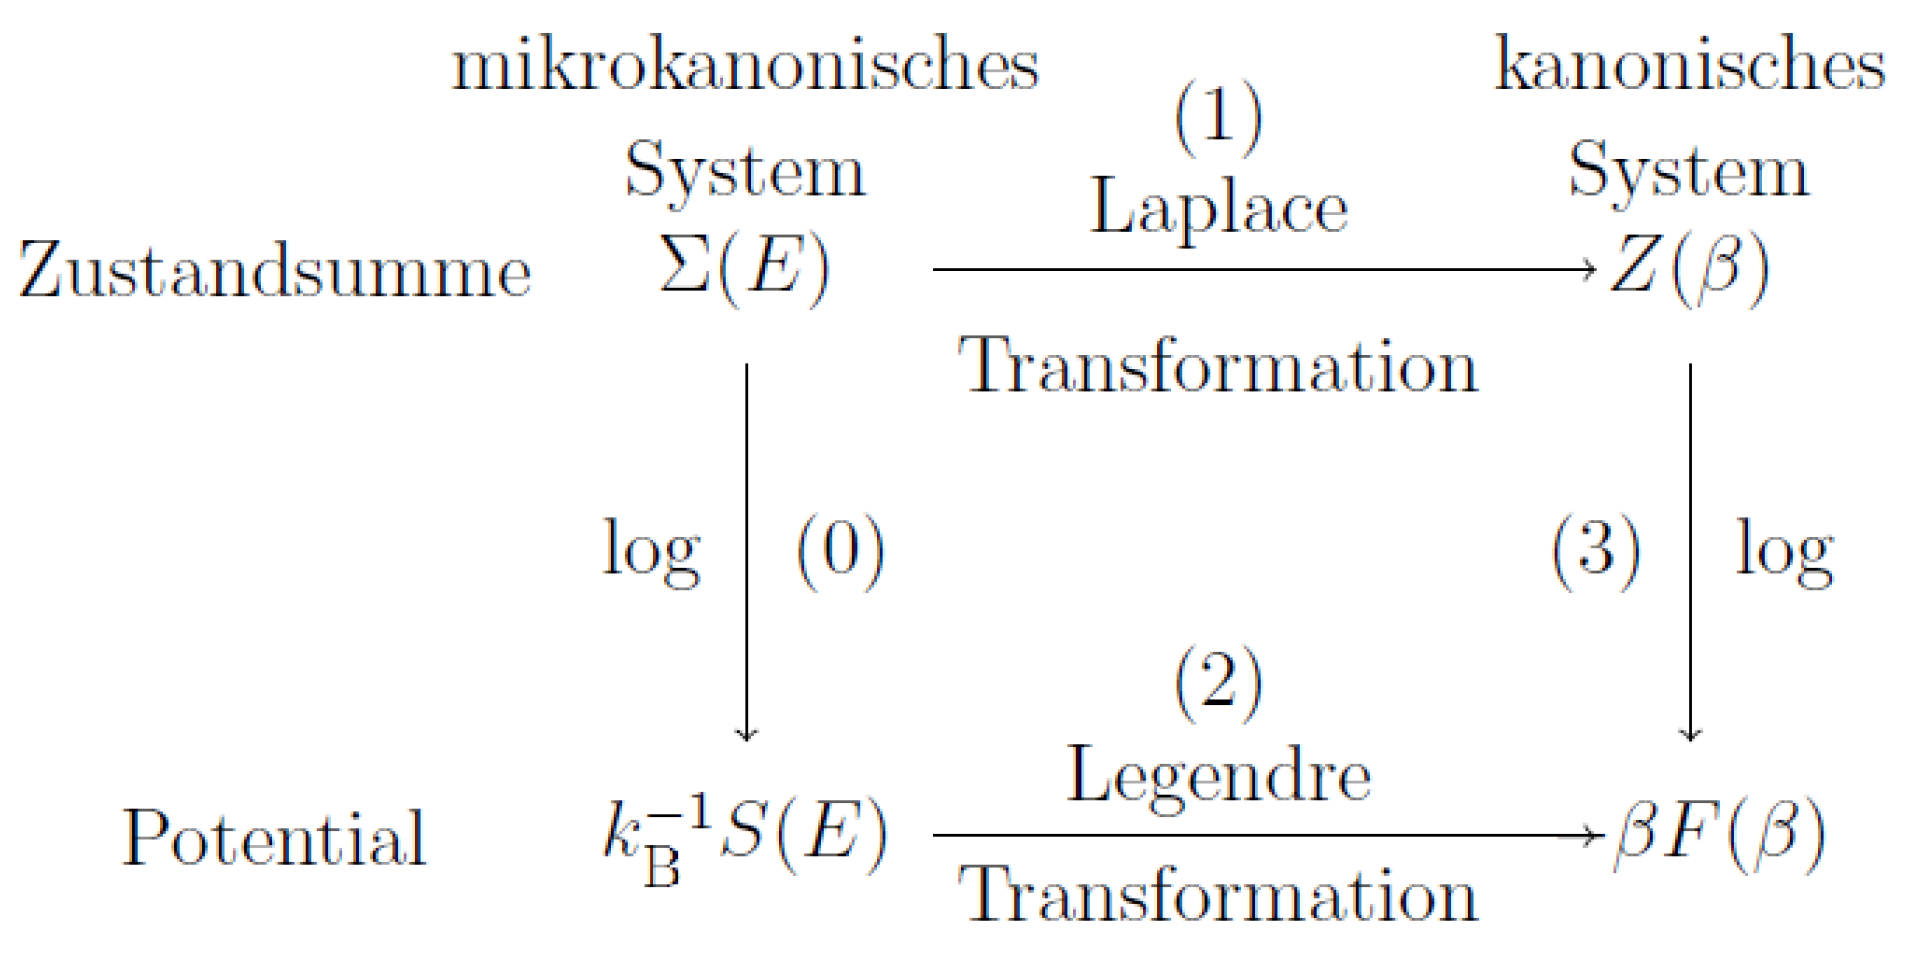
\includegraphics[width=0.3\textwidth]{Bilder/Aequivalenz_der_Gesamtheiten.png}
\end{figure}

Mittels Legendre Transformation erhalten wir:
\begin{align*}
    - \beta F_{mikro} (\beta) = - \beta \inf_S (U(S) - T S)
    = \sup_E (k_B^{-1} S_{mikro} (E) - \beta E)
\end{align*}
Wobei $S_{mikro}$ jene Entropie ist, welche aus dem mikrokanonischen Ensemble
hergeleitet wurde. Das Supremum wird angenommen für
\begin{align*}
    k_B^{-1} \frac{\partial S_{mikro}}{\partial E} = \beta
\end{align*}
Die kanonische Zustandssumme wird berechnet durch
\begin{align*}
    Z(\beta) &= \int dE \ d^{-\beta E} \Sigma(E)
    \equiv \int dE \ d^{g(E)}
    \\
    g(E) &= -\beta E + \log(\Sigma(E)) = - \beta E + k_B^{-1} S_{mikro} (E)
    \\
    g'(E) &= - \beta + k_B^{-1} \frac{\partial S_{mikro}}{\partial E}
    \\
    g''(E) &= k_B^{-1} \frac{\partial^2 S_{mikro}}{\partial E^2} = \mathcal{O}(1/N)
\end{align*}
Der grösste Beitrag zum Integral befindet sich bei der Energie $E=E_0$, wo
$g'(E_0) = 0$, d.h. wo
\begin{align*}
    k_B^{-1} \frac{\partial S_{mikro}}{\partial E} \Big|_{E_0} = \beta
\end{align*}
Mit der Näherung
\begin{align*}
    g(E) \approx g(E_0) + \frac{1}{2} g''(E_0) (E-E_0)^2
\end{align*}
wenden wir die Sattelpunkapproximation an und erhalten:
\begin{align*}
    Z(\beta) &\approx e^{-\beta E_0 + k_B^{-1} S_{mikro}(E_0)}
        \int dE \ e^{\frac{1}{2} g''(E_0)(E-E_0)^2}
    \\
    &= e^{-\beta F_{mikro}(\beta)} \underbrace{\mathcal{O} (\abs{g''(E_0)}^{-1/2})}_{= \mathcal{O}\klammer{N^{\frac{1}{2}}}}
\end{align*}
Somit ist
\begin{align*}
    F(\beta) \equiv - \beta^{-1} \log(Z(\beta)) = F_{mikro} (\beta) + \mathcal{O} \klammer{\log(N)}
\end{align*}

\subsection{Äquivalenz der Entropien}

Betrachte die informationstheoretische Entropie und die Statistische-Mechanik
Entropie. Wir betrachten nun den Grenzfall wo wir $\omega \rightarrow p$
diskretisieren.
\begin{align*}
    p(x) = \int_{\sigma(x)} \omega \ dx
    \approx \omega(x) \int_\sigma dx
    = \omega(x) h^{3N}
\end{align*}
wobei $\sigma \subset \Gamma_N$ von Volumen $h^{3N}$, d.h. $\int_\sigma dx = h^{3N}$.
$\sigma$ ist die kleinste Einheit die man betrachten kann. D.h. $\omega$ kann sich
darauf nicht ändern, bzw macht keinen Sinn. Damit folgt:
\begin{align*}
    S_{SM} (\omega) &= - k_B \sum_x h^{3N} \omega(x) \ln \klammer{\omega(x) h^{3N}}
    = - k_B \sum_x p(x) \ln \klammer{p(x)}
    \\
    &= k_B \ln(2) S_{IT} (p)
\end{align*}

Für ein 1-atomiges ideales Gas gilt: Bei einem Prozess bei dem $U_0 \rightarrow
U$ und $V_0 \rightarrow V$ ist
\begin{align*}
    S_{SM} &= k_B N \klammer{\frac{3}{2} + \log \klammer{\klammer{\frac{4 \pi m}{3}}^{3/2} \frac{1}{h^3}}}
        + k_B N \frac{3}{2} \log\klammer{\frac{E}{N}}
        \\ &\hspace{10pt}+ k_B N \log(V)
    \\
    \Delta S_{SM} &= k_B N \frac{3}{2} \log \klammer{\frac{U}{U_0}} + k_B N
        \log \klammer{\frac{V}{V_0}}
    \\
    \Delta S_{p} &= n \klammer{\int_{T_0}^T c_V \frac{dT}{T} + \int_{V_0}^V R \frac{dV}{V}}
    \\
    &= n c_v \log \klammer{\frac{U}{U_0}} + n R \log\klammer{\frac{V}{V_0}}
    \\
    \Rightarrow \hspace{5pt}
    R &= k_B \frac{N}{n} = k_B N_A
    \\
    c_v &= k_B \frac{N}{n} \frac{3}{2} = \frac{3}{2} R
\end{align*}
Wenn wir den Fall betrachten wo wir zwei Behälter mit jeweils $N$ Atomen und
Volumen $V$ zu einem Behälter mit $2N$ Teilchen und Volumen $2V$ zusammenführen
erhalten wir
\begin{align*}
    \Delta S_{p} &= 2N k_B \log(2N) - 2 N k_B \log(N) = 2N k_B \log(2)
    \\
    \Delta S_{SM} &= k_B 2N \log(2V) - 2 k_B N \log(V) = 2N k_B \log(2)
\end{align*}
Wir sehen, dass die SM Entropie derjenigen Entropie entspricht, wenn wir
annehmen, dass jedes Atom unterscheidbar ist.

Der einzige Term in der SM Entropie welcher nicht extensiv ist, ist $k_B N
\log(V)$. Wir nennen diesen Teil auch die Mischentropie. Falls wir annehmen,
dass die Teilchen ununterscheidbar sind, verschwindet dieser Term.


\subsubsection{Beweis der Äquivalenz}

Die Differenz der phenomenologischen Entropie wird durch einen Prozess $p$
beschrieben der ein System vom Zustand $\sigma_1$ in den Zustand $\sigma_2$
überführt: $\Delta S^p (p)$. Die Entropie der statistischen Mechanik nimmt
eine Wahrscheinlichkeitsverteilung $\omega$ als Argument: $S^{SM} (\omega)$.
Wir können mittels Gibbs'schem Variationsprinzip von $\sigma$ auf $\omega
= \omega(\sigma)$. Hierbei ist gemeint, dass $s^{SM}(\omega)$ maximiert wird
unter der Randbedingung $\sigma$. Wir haben bereits festgestellt, dass nur
Entropie Differenzen relevant sind. Wir wollen also zeigen, dass
\begin{align*}
    \Delta S^p (\sigma_1 \rightarrow \sigma_2) =
    S^{SM} (\omega(\sigma_2)) - S^{SM} (\omega(\sigma_1)).
\end{align*}
Wir bemerken ausserdem, dass der Referenzpunkt $S^{SM}(\omega_0) = 0$
von der Wahl von $h$ abhängt.
\begin{align*}
    \overline{S}^{SM} (\omega) &=
    - k_B \int dx \ \omega(x) \log \klammer{\omega(x) \overline{h}^{3N}}
    \\
    &= - k_B \int dx \ \omega(x) \log \klammer{\omega(x) h^{3N}}
    \\ &\hspace{20pt} - k_B \int dx \ \omega(x) \log \klammer{\klammer{\frac{\overline{h}}{h}}^{3N}}
    \\
    &= S^{SM} (\omega) - k_B 3N \klammer{\log(\overline{h}) - \log(h)}
\end{align*}
Weiter kann bewiesen werden, dass $S^{SM} (\omega)$ erhalten ist unter einem
Hamiltonischen Fluss $\phi_t$: $S^{SM} (\omega) = S^{SM} (\omega_t)$. Ausserdem
gelten die folgenden Eigenschaften:
\begin{enumerate}[(i)]
    \item $S^{SM}$ ist konkav mit WSK $p_0$ im Zst $\omega_0$ und mit Wsk
        $p_1$ im Zst $\omega_1$: $S^{SM} (p_0 \omega_0 + p_1 \omega_1) \geq
        p_0 S^{SM} (\omega_0) + p_1 S^{SM} (\omega_1)$.
    \item $S^{SM}$ ist additiv für unabhängige Systeme:
        $S^{SM} (\omega_A \times \omega_B) = S^{SM} (\omega_A) + S^{SM} (\omega_B)$
\end{enumerate}

Betrachte ein System mit Volumen $V$ und $N$ Teilchen welche durch eine Wand
in der linken Hälfte der Box gehalten werden. Betrachte nun den Prozess bei
dem die Wand entfernt wird. Die Entropie differenz ist dann gegeben als
\begin{align*}
    \Delta S^{IT} &= S^{IT}(\omega') - S^{IT}(\omega)
    \\
    &= \log_2 \klammer{V^N \int_{\geschwungeneklammer{H(p) = E}}}
        - \log_2 \klammer{\klammer{\frac{V}{2}}^N \int_{\geschwungeneklammer{H(p) = E}}}
    \\
    &= - \log_2 \klammer{\klammer{\frac{1}{2}}^N} = N 
\end{align*}
Hier ist $\omega$ die Wsk.verteilung vor dem Entfernen der Wand und $\omega'$
die Wsk.verteilung nach dem Entfernen der Wand. Allgemeiner gilt das folgende

\begin{theorem}
    Für jeden adiabatischen Prozess $\omega \rightarrow \omega'$ gilt immer
    \begin{align*}
        S^{SM} (\omega') \geq S^{SM} (\omega)
    \end{align*}
\end{theorem}

Im folgenden betrachten wir ein System wie oben mit $N=1$. D.h. wir sind im
gleichen Setup wie beim Gibbs'schen Paradox. Wir wählen den Referenzpunkt
der Entropie so, dass die Entropie der Systeme $M0$ und $M1$ bei denen man weiss
ob sich das Teilchen links oder rechts der Wand befindet Entropie $0$ hat. Nach
obiger Information über $\Delta S^{IT}$ folgt, dass das System $M?$ bei dem das
Teilchen mit $50 \%$-iger Wsk links oder rechts von der Wand ist, die Entropie
$1$ ist. Wir erinnern uns an die Betrachtung beim Gibbs'schen Paradox und stellen
fest, dass die Arbeit die für die Initialisierung $r$ benötigt wird um das System
$M?$ in entweder $M0$ oder $M1$ überzuführen gerade $W(r) = k_B T \log(2)$ ist.
Somit folgt für die Entropieänderung bei der Messung, dass
\begin{align*}
    \Delta S_M^p (r) = \frac{\Delta Q}{T} = - \frac{W}{T} = - k_b \log(2)
\end{align*}
Sei $K$ ein System auf dem ein reversibler Prozess $p$ das System vom
Zustand $\sigma_1$ in den Zustand $\sigma_2$ überführt. Die Entropieänderung
bei diesem Prozess ist gegeben als
\begin{align*}
    \Delta S_K^p (p) = \frac{\Delta Q_K (p)}{T} = S^p (\sigma_2) - S^p (\sigma_1)
\end{align*}
Betrachte nun das
System $K$, gekoppelt an ein Wärmereservoir $R$ bei Temperatur $T$, welches
wiederum an $\lambda$ viele Memorysysteme $M$ gekoppelt ist, was wir als
$M^\lambda$ schreiben. Ein Memorysystem ist ein Bit. Wir betrachten nun den
Prozess $r^\lambda \circ p$ der den Prozess $p$ ausführt und das Memorysystem
$M^\lambda$ resettet. Als $\lambda$ wählen wir nun
\begin{align*}
    \lambda = \frac{\Delta S_K^p}{k_B \ln(2)}
\end{align*}
Nun folgt:
\begin{align*}
    \Delta Q_R (p)
    &= - \Delta Q_K (p)
    = - T \Delta S_K^p (p)
    = - T \lambda k_B \ln(2)
    \\
    &= - \lambda T k_B \ln(2)
    = \lambda \Delta Q_M (r)
    = \Delta Q_{M^\lambda} (r^\lambda)
    \\
    &= - \Delta Q_R (r^\lambda)
\end{align*}
Somit folgt:
\begin{align*}
    \Delta Q_R (r^\lambda \circ p) = 0
\end{align*}
Da es sich um einen adiabatischen Prozess handelt, muss gelten
$\Delta S_{KRM}^{IT} (r^\lambda \circ p) \geq 0$. Daraus folgt:
\begin{align*}
    S_K^{IT} (\omega(\sigma_2)) + S_{M^\lambda} (M0^\lambda) + S_R
    &\geq
    S_K^{IT} (\omega(\sigma_1)) + S_{M^\lambda} (M?^\lambda) + S_R
    \\
    S_K^{IT} (\omega(\sigma_2)) - S_K^{IT} (\omega(\sigma_1))
    &\geq
    \lambda \klammer{S_{M}^{IT} (M?) - S_{M}^{IT} (M0)} = \lambda
    \\
    \Delta S_K^{IT}
    &\geq \frac{\Delta S_K^p}{k_B \ln(2)}
\end{align*}
Da der Prozess reversibel ist, gilt Gleichheit. Also folgt:
\begin{align*}
    \Delta S_K^p = k_B \log(2) \Delta S_K^{IT}
\end{align*}
\qed
